\documentclass[12pt,a4paper,oneside]{report}

% Essential Packages
\usepackage{setspace}
\usepackage{amsmath}
\usepackage{graphicx}
\usepackage{listings}
\usepackage{geometry}
\usepackage{xcolor}
\usepackage{hyperref}
\usepackage{booktabs}
\usepackage{float}
\usepackage{caption}

% Packages for Flowcharts
\usepackage{tikz}
\usetikzlibrary{shapes.geometric, arrows, positioning}

% Page Geometry & Spacing
\geometry{a4paper, margin=1in}
\setstretch{1.5}

% Code Listing Styles
\definecolor{codegreen}{rgb}{0,0.6,0}
\definecolor{codegray}{rgb}{0.5,0.5,0.5}
\definecolor{codepurple}{rgb}{0.58,0,0.82}
\definecolor{backcolour}{rgb}{0.95,0.95,0.92}

\lstdefinestyle{mystyle}{
    backgroundcolor=\color{backcolour},
    commentstyle=\color{codegreen},
    keywordstyle=\color{magenta},
    numberstyle=\tiny\color{codegray},
    stringstyle=\color{codepurple},
    basicstyle=\ttfamily\footnotesize,
    breakatwhitespace=false,
    breaklines=true,
    captionpos=b,
    keepspaces=true,
    numbers=left,
    numbersep=5pt,
    showspaces=false,
    showstringspaces=false,
    showtabs=false,
    tabsize=2
}
\lstset{style=mystyle}

% Improved TikZ Flowchart Styles
\tikzstyle{startstop} = [rectangle, rounded corners, minimum width=3.5cm, minimum height=1cm, text centered, draw=black, fill=blue!15, font=\small\bfseries]
\tikzstyle{io} = [trapezium, trapezium left angle=75, trapezium right angle=105, minimum width=3.5cm, minimum height=1cm, text centered, draw=black, fill=yellow!20, font=\small]
\tikzstyle{process} = [rectangle, minimum width=3.5cm, minimum height=1cm, text centered, draw=black, fill=orange!15, font=\small]
\tikzstyle{decision} = [diamond, minimum width=3.5cm, minimum height=1.2cm, text centered, draw=black, fill=green!15, font=\small]
\tikzstyle{arrow} = [thick,->,>=stealth]

\begin{document}

% ---------------------------------------------------------
% FRONT MATTER
% ---------------------------------------------------------
\pagenumbering{roman}

% Title Page
\begin{titlepage}
    \begin{center}
        \vspace*{1cm}
        \Large
        \textbf{INDIAN INSTITUTE OF TECHNOLOGY JODHPUR}
        
        \vspace{1cm}
        \large
        SUMMER RESEARCH INTERNSHIP 2026
        
        \vspace{1.5cm}
        % \includegraphics[width=4cm]{iitj_logo.png}
        \vspace{1.5cm}
        
        \Large
        INTERNSHIP REPORT
        
        \vspace{1.5cm}
        \Huge
        \textbf{Development of an IoT-Based Smart Health and Location Monitoring System}
        
        \vspace{1.5cm}
        \large
        Submitted in partial fulfillment of the requirements for the\\
        Internship
        
        \vspace{1.5cm}
        \Large
        By\\
        \textbf{Suyash Srivastav}\\
        B.Tech 2nd Year, Electronics and Communication Engineering (ECE)\\
        Gati Shakti Vishwavidyalaya, Vadodara, Gujarat
        
        \vfill
        
        \Large
        Under the Supervision of\\
        \textbf{Dr. Akshay Moudgil, Assistant Professor}
        
        \vspace{1.5cm}
        \large
        Department of Electrical Engineering\\
        Indian Institute of Technology Jodhpur\\
        May--July 2026
    \end{center}
\end{titlepage}

% Declaration
\chapter*{Declaration}
\addcontentsline{toc}{chapter}{Declaration}
I hereby declare that the work presented in this internship report titled ``Development of an IoT-Based Smart Health and Location Monitoring System'' is an authentic record of the work carried out by me during my internship at the Indian Institute of Technology Jodhpur, under the guidance of Dr. Akshay Moudgil. 

This project was executed in three distinct phases, involving sensor testing, ESP32 integration, and Raspberry Pi 5 setup. The work reported herein has not been submitted, in part or in full, to any other institute or university for the award of any degree or diploma. All sources of information used in this report have been duly acknowledged.
\vspace{2cm}

\noindent Place: Jodhpur\\
Date: 08 July 2026 \hfill \textbf{Suyash Srivastav}

% Certificate
\chapter*{Certificate}
\addcontentsline{toc}{chapter}{Certificate}
This is to certify that the internship report entitled ``Development of an IoT-Based Smart Health and Location Monitoring System'' is a bona fide record of the internship work carried out by \textbf{Suyash Srivastav} at the Indian Institute of Technology Jodhpur, under my supervision, during the period May 10 to July 10, 2026.

The work presented in this report is satisfactory for submission as part of the internship requirement.
\vspace{3cm}

\noindent \rule{6cm}{0.4pt}\\
\textbf{Dr. Akshay Moudgil}\\
Assistant Professor, Electrical Engineering Department\\
Indian Institute of Technology Jodhpur

% Acknowledgement
\chapter*{Acknowledgement}
\addcontentsline{toc}{chapter}{Acknowledgement}
I would like to express my sincere gratitude to Dr. Akshay Moudgil, Assistant Professor, Indian Institute of Technology Jodhpur, for providing me the opportunity to carry out this internship. His guidance and suggestions were very helpful throughout the duration of the project.

I am also thankful to the research scholars and laboratory staff of the electrical engineering department for their support during the hardware assembly and testing phases, and for granting access to the laboratory facilities required for this work.

I would further like to thank the Indian Institute of Technology Jodhpur for providing a great research environment. Finally, I extend my thanks to my family, my friends, and my home institution, Gati Shakti Vishwavidyalaya, for their continued support.

\vspace{1.5cm}
\noindent \textbf{Suyash Srivastav}

% Abstract
\chapter*{Abstract}
\addcontentsline{toc}{chapter}{Abstract}
This report details the development of an Internet of Things (IoT) based Smart Health and Location Monitoring System. The project was carried out in three main phases to make debugging and integration easier. 

\textbf{Phase 1} focused on testing and calibrating the individual sensors: the MAX30102 for heart rate and SpO2, the MLX90614 for body temperature, and the NEO-6M GPS module for location tracking. \textbf{Phase 2} involved integrating these sensors with an ESP32 microcontroller, which sent the data over Wi-Fi using the MQTT protocol. A web dashboard was also built using React.js and Firebase, and hosted on Vercel to view the data. \textbf{Phase 3} improved the system by upgrading the main controller to a Raspberry Pi 5 to handle more complex coding tasks. In this final phase, the circuit was moved from a breadboard to a soldered Zero PCB (perfboard) to make it more compact. A mobile app was also created using React Native (Expo Go) so users could monitor the data from their phones. 

This report explains the hardware setup, the math behind the signal processing, the software logic, and the final results obtained during the internship. 

\tableofcontents
\listoffigures
\listoftables

\clearpage
% ---------------------------------------------------------
% CORE BODY
% ---------------------------------------------------------
\pagenumbering{arabic}

% --- CHAPTER 1 ---
\chapter{Introduction}
\section{Background and Motivation}
Low-cost microcontrollers and wireless modules have made it easier to build wearable IoT devices that can monitor health and environmental conditions. People increasingly need devices that can track vital signs and geographic locations remotely. This project aims to build a practical monitoring device that can collect health data and GPS coordinates, and display them on a web or mobile dashboard.

\section{Existing Solutions vs. Proposed System}
Commercially available health monitoring devices, such as the Apple Watch or Garmin smartwatches, offer excellent physiological tracking. However, these systems come with significant drawbacks for researchers and independent developers: they are highly expensive, their internal data processing algorithms are proprietary, and they lock the user's data within closed ecosystems. 

This project proposes a custom, open-architecture alternative. By building the device from off-the-shelf components, the total cost is kept low. More importantly, it provides unrestricted access to the raw sensor data, allowing for custom signal processing and full ownership of the data pipeline on Firebase.

\section{Problem Statement}
Connecting multiple sensors (using I2C and UART protocols) to a single microcontroller requires careful wiring and programming. The device needs to read heart rate, body temperature, and location, process the data, and send it to a server. The hardware also needs to be compact enough to be worn, moving from a messy breadboard setup to a soldered PCB, and the software needs a proper user interface.

\section{Project Phasing}
To keep the development organized, the project was divided into three phases:
\begin{enumerate}
    \item \textbf{Phase 1:} Testing individual sensors and writing basic Arduino code.
    \item \textbf{Phase 2:} Connecting the sensors to an ESP32, setting up MQTT, and building a Vercel web dashboard.
    \item \textbf{Phase 3:} Upgrading to a Raspberry Pi 5, soldering the components onto a Zero PCB, and making an Expo Go mobile app.
\end{enumerate}


% --- CHAPTER 2 ---
\chapter{Phase 1: Sensor Testing and Characterization}
Before putting everything together, each sensor was tested separately on a breadboard. This helped verify that the sensors worked, check their communication protocols (I2C/UART), and write the basic code for them.

\section{MAX30102 Pulse Oximeter and Heart Rate Sensor}
The MAX30102 is a sensor module that measures heart rate and blood oxygen levels. It connects via I2C and uses photoplethysmography (PPG) to detect changes in blood volume. It gives raw optical data that is used to calculate beats per minute (BPM).

\begin{figure}[H]
    \centering
    % Placeholder for MAX30102 testing image
    \rule{0.6\textwidth}{0.3\textheight}
    \caption{Breadboard testing setup of the MAX30102 sensor.}
    \label{fig:max30102_test}
\end{figure}

\begin{lstlisting}[language=C++, caption=Testing Code for MAX30102 (Arduino IDE)]
#include <Wire.h>
#include "MAX30105.h"
#include "heartRate.h"

MAX30105 particleSensor;
const byte RATE_SIZE = 4;
byte rates[RATE_SIZE];
byte rateSpot = 0;
long lastBeat = 0;
float beatsPerMinute;
int beatAvg;

void setup() {
  Serial.begin(115200);
  if (!particleSensor.begin(Wire, I2C_SPEED_FAST)) {
    Serial.println("MAX30102 was not found. Please check wiring.");
    while (1);
  }
  particleSensor.setup();
  particleSensor.setPulseAmplitudeRed(0x0A);
}

void loop() {
  long irValue = particleSensor.getIR();
  if (checkForBeat(irValue) == true) {
    long delta = millis() - lastBeat;
    lastBeat = millis();
    beatsPerMinute = 60 / (delta / 1000.0);
    if (beatsPerMinute < 255 && beatsPerMinute > 20) {
      rates[rateSpot++] = (byte)beatsPerMinute;
      rateSpot %= RATE_SIZE;
      beatAvg = 0;
      for (byte x = 0 ; x < RATE_SIZE ; x++) beatAvg += rates[x];
      beatAvg /= RATE_SIZE;
    }
  }
  Serial.print("IR = ");
  Serial.print(irValue);
  Serial.print(", BPM = ");
  Serial.println(beatAvg);
}
\end{lstlisting}

\section{MLX90614 Infrared Temperature Sensor}
The MLX90614 is a non-contact infrared thermometer. It also uses I2C and reads both the surrounding room temperature and the temperature of the object it is pointed at, which is useful for checking body temperature without skin contact.

\begin{figure}[H]
    \centering
    % Placeholder for MLX90614 testing image
    \rule{0.6\textwidth}{0.3\textheight}
    \caption{Breadboard testing of the MLX90614 IR temperature sensor.}
    \label{fig:mlx_test}
\end{figure}

\section{NEO-6M GPS Module}
The NEO-6M provides standard location data (NMEA format) over a UART serial connection. The \texttt{SoftwareSerial} library was used on the microcontroller to read the latitude and longitude coordinates.

\begin{figure}[H]
    \centering
    % Placeholder for NEO-6M testing image
    \rule{0.6\textwidth}{0.3\textheight}
    \caption{Breadboard testing and satellite fix of the NEO-6M GPS module.}
    \label{fig:gps_test}
\end{figure}

% --- CHAPTER 3 ---
\chapter{Mathematical Signal Processing}
To get accurate heart rate and SpO2 readings from the MAX30102, the raw optical data needs to be processed using some basic math in the code.

\section{Photoplethysmography and the Beer-Lambert Law}
Calculating blood oxygen (SpO2) depends on how oxygenated hemoglobin ($HbO_2$) and deoxygenated hemoglobin ($Hb$) absorb light differently. This follows the Beer-Lambert Law, which states that the absorbance $A$ of light passing through a material is:
\begin{equation}
    A = \ln\left(\frac{I_{in}}{I_{out}}\right) = \varepsilon \cdot c \cdot d
\end{equation}
Here, $\varepsilon$ is how much light the blood absorbs, $c$ is the concentration of hemoglobin, and $d$ is the distance the light travels through the tissue.

\section{The Ratio of Ratios Algorithm}
Because we don't know the exact distance $d$ the light travels through the skin, the code separates the changing part of the signal (the AC component) from the steady baseline (the DC component) for both the Red and Infrared (IR) LEDs.

This gives us the "Ratio of Ratios" ($R$):
\begin{equation}
    R = \frac{\left( \frac{AC_{red}}{DC_{red}} \right)}{\left( \frac{AC_{ir}}{DC_{ir}} \right)}
\end{equation}
Once $R$ is calculated in the code, a standard linear formula is used to estimate the SpO2 percentage:
\begin{equation}
    SpO_2 (\%) = 110 - 25 \cdot R
\end{equation}
This calculation is done continuously on the microcontroller before any data is sent over the internet.


% --- CHAPTER 4 ---
\chapter{Phase 2: ESP32 System Integration}
\section{System Architecture}
After testing the individual components, they were connected to an ESP32 microcontroller. The ESP32 reads the MAX30102 and MLX90614 using the I2C pins, and the NEO-6M GPS using the UART pins. 

\section{Hardware Pin Mapping}
To ensure reliable communication, the sensors were wired to the ESP32 using the specific GPIO pins listed in Table~\ref{tab:esp32_pins}.

\begin{table}[H]
\centering
\begin{tabular}{@{}llcc@{}}
\toprule
\textbf{Sensor / Module} & \textbf{Pin Function} & \textbf{ESP32 GPIO} & \textbf{Logic Level} \\ \midrule
MAX30102 (PPG)           & SDA (I2C Data)        & GPIO 21             & 3.3V                 \\
MAX30102 (PPG)           & SCL (I2C Clock)       & GPIO 22             & 3.3V                 \\
MLX90614 (Temp)          & SDA (I2C Data)        & GPIO 21             & 3.3V                 \\
MLX90614 (Temp)          & SCL (I2C Clock)       & GPIO 22             & 3.3V                 \\
NEO-6M (GPS)             & TX (UART Transmit)    & GPIO 16 (RX2)       & 3.3V                 \\
NEO-6M (GPS)             & RX (UART Receive)     & GPIO 17 (TX2)       & 3.3V                 \\ \bottomrule
\end{tabular}
\caption{Hardware pin mapping for the ESP32 integration phase.}
\label{tab:esp32_pins}
\end{table}

\section{Data Structuring and JSON Payloads}
Before transmitting data over MQTT, the edge device packages the readings into a structured JSON (JavaScript Object Notation) format. This makes the data lightweight and easy for the web dashboard to parse. An example payload transmitted by the device is shown below:

\begin{lstlisting}[language=java, caption=Example JSON telemetry payload sent to the cloud.]
{
  "device_id": "esp32_node_01",
  "bpm": 76,
  "spo2": 98,
  "temp_ambient_c": 32.1,
  "temp_object_c": 36.5,
  "gps": {
    "lat": 26.2389,
    "lon": 73.0243,
    "isValid": true
  },
  "timestamp": 1688754321
}
\end{lstlisting}

\section{Vercel Frontend Web Dashboard}
A web dashboard was built to display the health and location data for the user. It was created using React.js and Node.js, and hosted on Vercel. Leaflet.js was used to show the GPS coordinates as a marker on an interactive map.


% --- CHAPTER 5 ---
\chapter{Software Architecture and Execution Flow}
To make sure the microcontroller doesn't get stuck while waiting for a network connection, a non-blocking code structure was used. Instead of using \texttt{delay()} which stops the whole program, the code checks the current time to decide if it should read a sensor or send data to the cloud.

The flowchart below shows the main loop running on the device.

\begin{figure}[H]
    \centering
    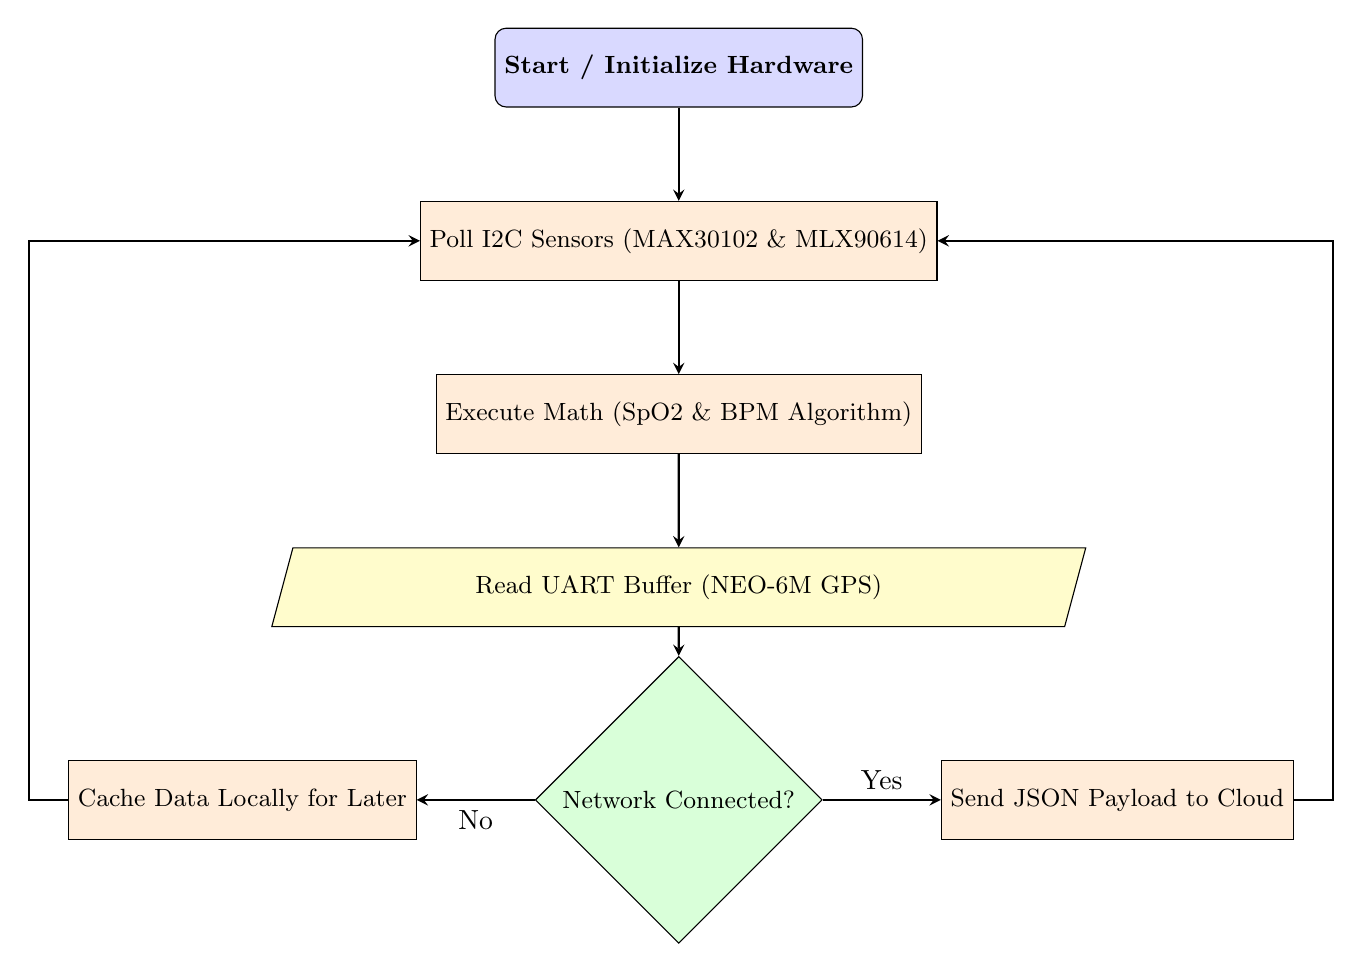
\begin{tikzpicture}[node distance=2.2cm, auto]
        % Nodes
        \node (start) [startstop] {Start / Initialize Hardware};
        \node (read_i2c) [process, below of=start] {Poll I2C Sensors (MAX30102 \& MLX90614)};
        \node (dsp) [process, below of=read_i2c] {Execute Math (SpO2 \& BPM Algorithm)};
        \node (read_uart) [io, below of=dsp] {Read UART Buffer (NEO-6M GPS)};
        \node (dec1) [decision, below of=read_uart, yshift=-0.5cm] {Network Connected?};
        \node (mqtt) [process, right=1.5cm of dec1] {Send JSON Payload to Cloud};
        \node (cache) [process, left=1.5cm of dec1] {Cache Data Locally for Later};
        
        % Arrows
        \draw [arrow] (start) -- (read_i2c);
        \draw [arrow] (read_i2c) -- (dsp);
        \draw [arrow] (dsp) -- (read_uart);
        \draw [arrow] (read_uart) -- (dec1);
        
        \draw [arrow] (dec1) -- node {Yes} (mqtt);
        \draw [arrow] (dec1) -- node {No} (cache);
        
        % FIXED loop back paths - routing outwards first to avoid overlapping nodes
        \draw [arrow] (mqtt.east) -- ++(0.5,0) |- (read_i2c.east);
        \draw [arrow] (cache.west) -- ++(-0.5,0) |- (read_i2c.west);
    \end{tikzpicture}
    \caption{Flowchart showing the main non-blocking software loop.}
    \label{fig:software_flow}
\end{figure}


% --- CHAPTER 6 ---
\chapter{Phase 3: Raspberry Pi 5 and Mobile App Integration}
\section{Migrating to Raspberry Pi 5}
To handle more data and run Python code easily, the main board was changed from an ESP32 to a Raspberry Pi 5. The Pi 5 has better processing capabilities, which allows it to use Python's \texttt{asyncio} library. This means it can read sensors and send data at the same time without freezing up.

\section{Hardware Pin Mapping (Pi 5)}
The migration to the Raspberry Pi 5 required a new wiring layout, as shown in Table~\ref{tab:pi5_pins}. 

\begin{table}[H]
\centering
\begin{tabular}{@{}llcc@{}}
\toprule
\textbf{Sensor / Module} & \textbf{Pin Function} & \textbf{Pi 5 Physical Pin} & \textbf{Pi 5 GPIO} \\ \midrule
MAX30102 (PPG)           & SDA (I2C 1)           & Pin 3                      & GPIO 2             \\
MAX30102 (PPG)           & SCL (I2C 1)           & Pin 5                      & GPIO 3             \\
MLX90614 (Temp)          & SDA (I2C 1)           & Pin 3                      & GPIO 2             \\
MLX90614 (Temp)          & SCL (I2C 1)           & Pin 5                      & GPIO 3             \\
NEO-6M (GPS)             & TX (UART)             & Pin 10                     & GPIO 15 (RXD)      \\
NEO-6M (GPS)             & RX (UART)             & Pin 8                      & GPIO 14 (TXD)      \\ \bottomrule
\end{tabular}
\caption{Hardware pin mapping for the Raspberry Pi 5 integration phase.}
\label{tab:pi5_pins}
\end{table}

\section{Zero PCB Fabrication and Miniaturization}
The breadboard circuit was too bulky, so the components were soldered onto a Zero PCB (perfboard). Because the Raspberry Pi 5 uses 3.3V logic and some sensors output 5V, logic level converters (MOSFETs) were used to step down the voltage and protect the Pi's pins. The final soldered board was much smaller and more stable.

\begin{figure}[H]
    \centering
    % Placeholder for PCB connection image
    \rule{0.7\textwidth}{0.35\textheight}
    \caption{Soldered Zero PCB layout with hardware connections for Phase 3.}
    \label{fig:pcb_layout}
\end{figure}

\section{Expo Go Mobile Application}
A mobile app was created using React Native and Expo Go to make it easier for users to check the data. The app connects to the Firebase database to get live updates. Expo made it simple to build the app for both Android and iOS devices, and the layout looks similar to the web dashboard.


% --- CHAPTER 7 ---
\chapter{System Challenges and Troubleshooting}
During the project, several hardware issues came up. Here is how they were fixed.

\section{Logic Level Voltage Mismatches}
\textbf{Challenge:} The Raspberry Pi 5 operates on 3.3V logic, but the NEO-6M GPS works better at 5V. Connecting a 5V signal directly to the Pi's RX pin can damage it. \\
\textbf{Solution:} Bidirectional logic level shifters (using BSS138 transistors) were placed between the sensors and the Pi. This safely dropped the 5V signals down to 3.3V before they reached the Pi.

\section{GPS Cold Start Latency}
\textbf{Challenge:} When testing outside, the NEO-6M GPS took a long time (3 to 5 minutes) to find satellites and get a lock. \\
\textbf{Solution:} A coin-cell battery was added to the GPS module. This kept the satellite data saved in memory when the power was off, allowing the GPS to get a "hot start" and find a lock in just a few seconds. The code was also updated to only send GPS data if it was valid.

\section{Motion Artifacts in PPG Sensing}
\textbf{Challenge:} The MAX30102 sensor is sensitive to movement. If the user moved around, the heart rate readings would jump to random high numbers. \\
\textbf{Solution:} A moving average filter was added to the code to smooth out the noise. Also, a limit was set in the code to ignore any heart rate values that were physically impossible (like anything above 220 BPM).


% --- CHAPTER 8 ---
\chapter{Results, Testing, and Dashboards}

\section{Sensor Accuracy and Experimental Data}
To verify the system's reliability, the sensors were tested against standard commercial devices. 
\begin{itemize}
    \item \textbf{Temperature Validation:} The MLX90614 readings were compared with a standard clinical digital thermometer. The sensor showed an accuracy variance of $\pm 0.3^\circ$C when placed at a 2 cm distance from the forehead.
    \item \textbf{GPS Lock Time:} Outdoors under a clear sky, the NEO-6M achieved a "hot start" satellite lock in an average of 12 seconds thanks to the backup battery, compared to over 3 minutes on a cold start.
\end{itemize}

\begin{figure}[H]
    \centering
    % Placeholder for a graph comparing the PPG sensor to a commercial smartwatch
    \rule{0.7\textwidth}{0.3\textheight}
    \caption{Graph comparing the custom PPG heart rate readings with a commercial smartwatch over a 60-second window.}
    \label{fig:bpm_graph}
\end{figure}

\section{Backend Database Validation}
Data transmitted from the device was successfully received and logged in the Firebase Realtime Database. The nested JSON structure allowed for fast querying and data retrieval.

\begin{figure}[H]
    \centering
    % Placeholder for Firebase Screenshot
    \rule{0.8\textwidth}{0.3\textheight}
    \caption{Screenshot of the Firebase Realtime Database showing live incoming JSON documents.}
    \label{fig:firebase_db}
\end{figure}

\section{Phase 2: Web Dashboard Results}
The React.js dashboard on Vercel successfully received data from the ESP32. The interface showed the live BPM, temperature, and updated the GPS location on the Leaflet.js map without any major delays.

\begin{figure}[H]
    \centering
    % Placeholder for Phase 2 Dashboard image
    \rule{0.8\textwidth}{0.35\textheight}
    \caption{Phase 2: React.js Web Dashboard hosted on Vercel.}
    \label{fig:phase2_dashboard}
\end{figure}

\section{Phase 3: Mobile App and PCB Results}
Moving to the Raspberry Pi 5 and the Zero PCB worked well. The final device size was significantly reduced compared to the breadboard version, making it much easier to carry. The Expo Go mobile app ran smoothly and displayed the live data correctly on mobile devices.

\begin{figure}[H]
    \centering
    % Placeholder for Phase 3 Mobile Dashboard image
    \rule{0.5\textwidth}{0.5\textheight}
    \caption{Phase 3: React Native Mobile Application running via Expo Go.}
    \label{fig:phase3_dashboard}
\end{figure}


% --- CHAPTER 9 ---
\chapter{Conclusion and Future Scope}
\section{Conclusion}
This project covered the complete development of an IoT-based Smart Health and Location Monitoring System. By splitting the work into three phases, it was easier to troubleshoot issues. Phase 1 verified that all sensors worked properly. Phase 2 showed that data could be sent over Wi-Fi to a web dashboard using an ESP32. Phase 3 improved the system by using a Raspberry Pi 5, a soldered Zero PCB, and a mobile app. The internship provided good hands-on experience with sensors, microcontrollers, soldering, and software development.

\section{Future Scope}
Possible improvements for the future include:
\begin{itemize}
    \item \textbf{Custom PCB:} Designing and printing a proper PCB using KiCad instead of hand-soldering a perfboard, which would make the device even smaller and more reliable.
    \item \textbf{Battery Power:} Adding a proper LiPo battery and charging circuit so the device can run on its own for hours without needing an external power bank.
    \item \textbf{Alert System:} Adding a feature to the app that sends an email or SMS alert if the heart rate or temperature goes outside a normal range.
\end{itemize}

\end{document}
